\chapter{An Overview of Snapstore}

Snapstore was created with two distinct groups of users in mind, non-technical users and technical users. In order to be an attractive system to technical users who use systems like Git, Snapstore needed to support the functionality of powerful version control systems. However, Snapstore also needed to have a smoother learning curve to promote quick startup and attract users who feel overwhelmed by complicated VCSs. 

We decided to create Snapstore with an opt-in strategy concerning complexity. Users can download Snapstore and get started right away with simple actions like file backup. Then, if desired, users can explore more advanced features of the system.

%Snapstore uses a simple user-based identification system. Once a user downloads Snapstore, they create an account with a username.

Snapstore operates within a specially designated Snapstore folder which is created upon opening the application for the first time. It is similar to the Dropbox folder; Snapstore only looks at files that are inside of it. Snapstore watches the user's filesystem for changes in order to respond with certain actions like creating snapshots (section 2.1.1). This allows users to use any editor with Snapstore. Also, the Snapstore folder that Snapstore creates does not need to remain the only folder used by the application. Snapstore can be opened using any folder as the Snapstore folder.

\section{Basic Features}

The basic features of Snapstore allow a single user to use the application like they would a file syncing system.

\subsection{Snapshots}

\textit{Snapshots} allow a user to persistently store all of their edits to a file over time. Whenever a file is saved to disk, a snapshot is created with the contents of that file and stored in the local repository. The type of each snapshot corresponds to the action that created it. Snapshots can be the result of a create, update, rename, delete, merge, or conflicting merge of a file. Users can retreive an old state of a file by finding the appropriate snapshot in the file's history.

Snapshots are created when a file is created, updtaed, deleted or renamed. Snapshots are also created when files are merged together. These snapshots are either the result of a successful merge or of a conflicting merge. Snapshots, then, can be one of six types: create, update, delete, rename, merge, or conflict.

When creating snapshots for a given file, Snapstore will add the snapshot to that file's \textit{snapshot graph}. This graph represents the history of the file and it shows each snapshot that was taken, along with its relationship to other snapshots of that file. A snapshot has one or more parents (the snapshot(s) taken before it), and it has a child (the snapshot taken after it). The only way a snapshot could have more than one parent is if it's a product of a merge of multiple snapshots. The first snapshot in a graph is called the \textit{root}, and the last snapshot in the graph is called the \textit{head}.

To show a sequence of snapshots from a file's history, navigate to that file within Snapstore's interface. Then, click on the file's name. The snapshot graph will appear at the top of the window. Each node in this graph is a snapshot, and the node on the far right is the head. By clicking on these nodes, the content of the snapshot will appear on the bottom-right of the window. After the correct snapshot is found, it's possible to revert to that snapshot by clicking ``Revert'', a button above the snapshot content. Reverting to a previous snapshot will create a new snapshot with the same content at the head position and alter the file's content to match the snapshot's content.

\subsection{Upstreams}

\textit{Upstreams} are used to synchronize the data of collaborators on a project. Whenever a user makes any changes to their Snapstore system, those changes are sent to the upstream and out to all other users who are collaborating with that user.

If two users are working together on a project, the upstream will synchronize their snapshots as they make them. In the case of multiple snapshots coming in to the upstream at the same time, the upstream will resolve the conflict and push the same ordering of snapshots to both users.

By default, the upstream is the Snapstore server, but users might want to change their upstream so their data passes through a known location. To do so, follow these steps:
\begin{enumerate}
  \item{Download the Snapstore server program onto the machine}
  \item{Run the Snapstore server on that machine}
  \item{Point the Snapstore client to that machine}
\end{enumerate}

\subsection{Local Repository}

The \textit{local repository} allows users to work without an active Internet connection. Whenever a user makes any changes to their Snapstore system that data is saved in the local repository. When connection is restored, Snapstore will push all new changes to the upstream.

\section{Advanced Features}

Snapstore's advanced features allow users to access the more powerful components of a version control system. They provide additional functionality that users might want when working on projects with complex version control requirements.

\subsection{Groups}

\textit{Groups} allow users to designate a collection of snapshots as related. When a user has a collection of snapshots they believe are related, even if they exist across multiple files, they can place them in a group. The user can then give this group a name.

A software team collaborating on a project might want to fix a syntax bug in their program. If one user makes a few snapshots in this process, they can then place them in a group and title it ``Fixed syntax bug''. Now, these snapshots and this group have all been shared with the other team members through the upstream. Team members can easily locate this group and inspect its snapshots to see how the bug was fixed. 

\subsection{Tags}

\textit{Tags} allow users to designate a group as a coherent point in development. The exact nature of a coherent point will differ from project to project, but in general this means a point in which the project is ready for further development. When a group of snapshots is particularly significant, such as project completion or a release of a piece of software, users can tag that group.

Tags can only be given to groups who have at most once snapshot per file. This is so that a the user can revert the state of their files using the tag. When this is done, every file that is in the group with that tag wil be reverted to the state described by the snapshots in that group.

For a software release, a user can tag the group of head snapshots ``Version 1.3'' to signify that the project is in a stable release state. Later, after more snapshots have been created, users can utilize this tag to revert the project to the group of snapshots tagged by ``Version 1.3''.

\subsection{Branches}

\textit{Branches} allow users to separate parallel lines of work. Whenever any data is created, it is saved within the user's current branch. Switching to a different branch will load all data associated with that branch, changing the user's filesystem as necessary. Branches can be merged together to combine parallel lines of work.

Snapstore provides a default branch called ``master'' on startup. A user can then create and use new branches to maintain multiple versions/releases of the same project, keep the development of major features isolated, and to give users the ability to try out experimental changes without affecting the main line \cite{RossoJackson}.

A branch can also be created by cloning an existing branch. Creating a clone involves choosing a branch to clone and selecting snapshots inside the original branch to bring over to the clone. For all snapshots that are cloned into the new branch, any groups associated those snapshots, and any tags associated with those groups, will be copied to the cloned branch.

\subsubsection{Sharing Branches}

When a branch is shared with another user, that branch's data is copied on that user's local repository. On a shared branch, when any user makes changes, those changes are immediately sent to the other user(s) associated with that shared branch. For example, one user might create a new snapshot on a file in the shared branch. That new snapshot is propagated to all collaborators on that branch and reflected in their snapshot graphs and on their filesystem.

When conflicts arise due to multiple users working on the same branch at the same time, Snapstore uses last-write wins rule. The last snapshot to reach the server will become the head snapshot for the file. Other snapshots are placed before the head snapshot in the snapshot graph. No snapshots are lost in the conflict, and the user can revert to a passed over snapshot easily.

Figure 2-1 illustrates an example of two user working on a shared branch. Snapshot graphs containing numbered snapshots are included for both users and for the upstream. Step 1 shows Alice and Bob's shared snapshot 1. In step 2, Alice makes snapshot 3 and Bob makes snapshot 2 simultaneously. In step 3, Alice's snapshot 3 makes it to the upstream first, so the upstream adds it to its snapshot graph. Bob's snapshot 2 tries to make it to the upsream in step 4, but it is rejected and snapshot 3 is sent back along with the rejection; 3 is inserted into Bob's snapshot graph. Bob's snapshot 2 finally makes it to the upstream in step 5, and it is propagated to Alice in step 6.

\begin{figure}
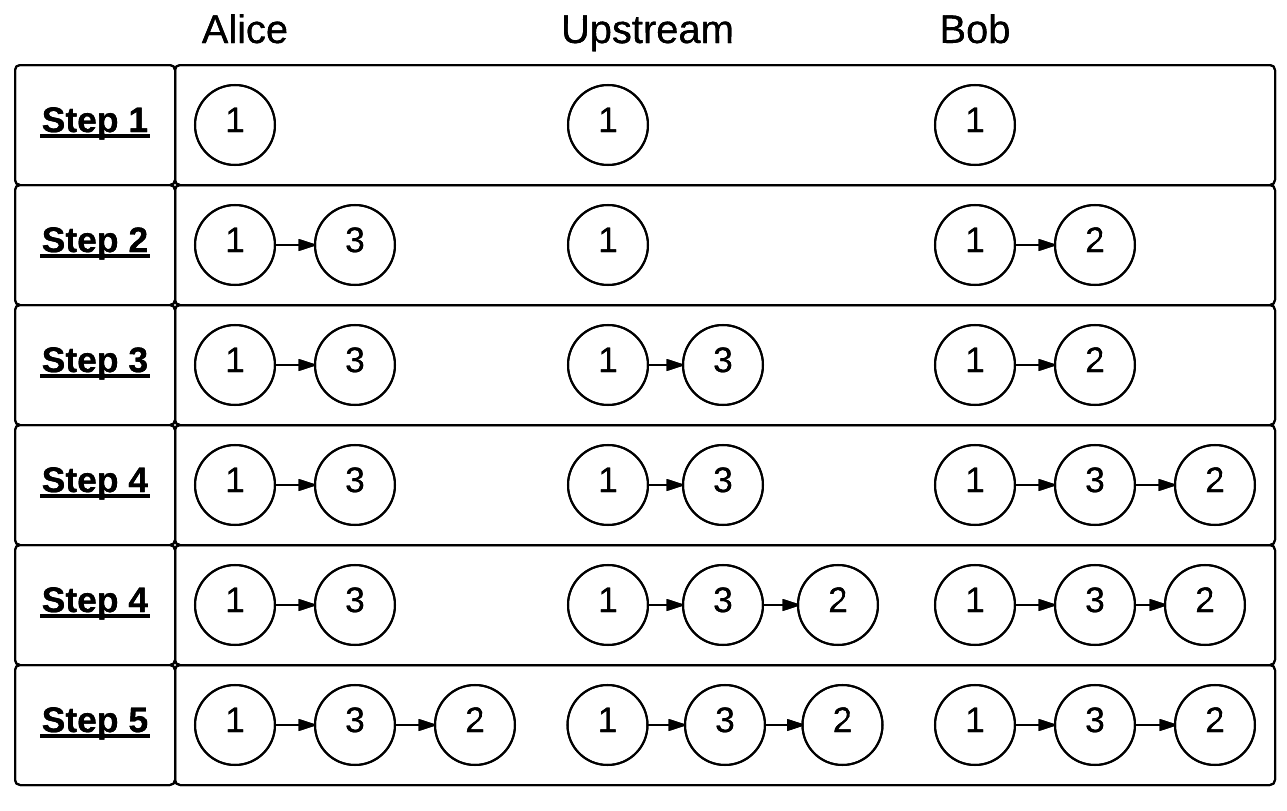
\includegraphics[max width= \linewidth]{Collaborating}
\caption{Conflicts being resolved on a shared branch.}
\label{arm:fig1}
\end{figure}

\subsubsection{Merging Branches}

Merging two branches compares the snapshot graphs in those two branches. If two snapshot graphs correspond to the same file, then a merge is performed using three way merge and their common ancestor. This will result in a merge snapshot with as many parents as there are snapshots being merged. If there is a merge conflict, then the resulting snapshot will be a conflict snapshot. Like in Git, a conflict snapshot's content will show where the conflict needs to be resolved. Unlike in Git, this merge snapshot is already on the server and saved, no conflict resolution is needed to continue working. By simply fixing the conflict and saving, a new snapshot is created that reflects the fix. Merging two branches will keep all of the group and tag data from both branches.

Figure 2-2 shows an overview of branch merging in Snapstore. In this image, the file id is shown next to the head snapshot for each snapshot graph. Once snapshot graphs are identified as corresponding to the same file id, their head snapshots are merged into a new snapshot, whose parents are the old head snapshots. Any snapshot graph that does not have a counterpart in the other branch will just be copied over to the merged branch.

\begin{figure}
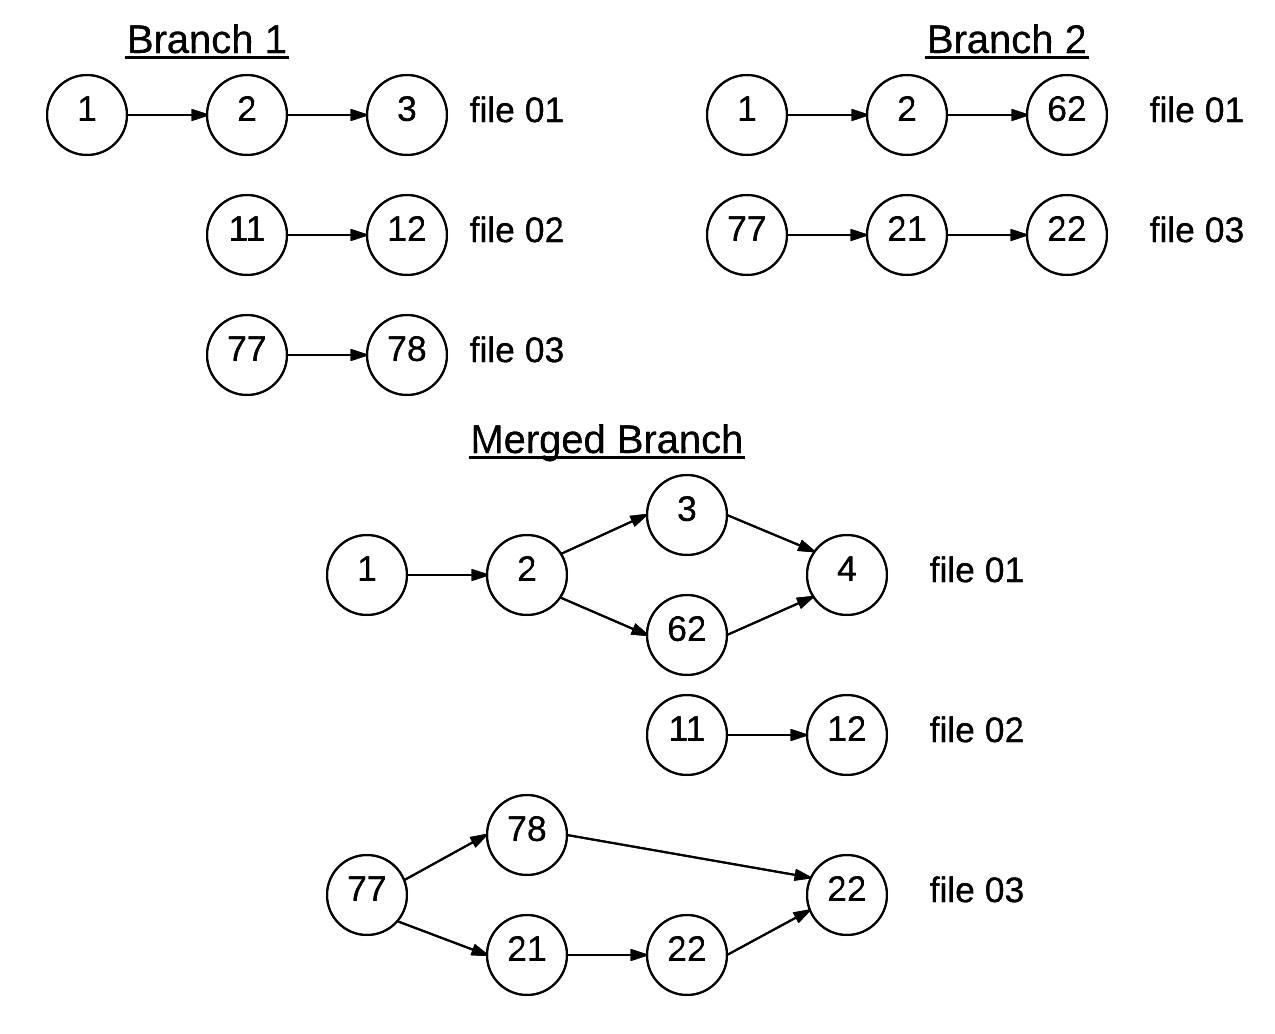
\includegraphics[max width= \linewidth]{Merging}
\caption{Merging two branches.}
\label{arm:fig1}
\end{figure}

\subsection{Use Cases}

\subsubsection{Single User on Multiple Computers}

A single user using more than one computer makes use of upstreams and local repositories. In this case, they are collaborating with themselves, on different computers with different local repositories. The user can work on computer $A$, saving changes to their local repository. When they open Snapstore on computer $B$, computer $A$'s local repository will push those changes to computer $B$ through the upstream.

\subsubsection{Project Management}

Effective project management can be done by creating multiple clones of the main project.

Imagine a web application project called ``webIt'' with four workers: a project manager, a front-end developer, and back-end developer, and a graphic artist. The project manager needed to break up the entire workspace to achieve two simultaenous goals. Though there are parts of the project were collaboration was essentiall, her first goal was to keep her employees away from parts of the project with which they had no part. The second goal was to be able to merge these various parts back into one complete and conflict-free project.

To accomplish these goals within Snapstore, the project manager would first create three clones of her ``webIt'' branch: ``front-end'', ``API'', and ``back-end''. The manager shares ``front-end'' branch with the front-end developer and the graphic artist, the ``API'' branch with the front and back-end developers, and the ``back-end'' branch with only the back-end developer. 

The project manager can keep an eye on each branch's progress because she has access to them; as each person creates new snapshots, they show up on her machine as well. Whenever the time comes for a new release, the project manager can merge her cloned branches with her ``webIt'' branch. 

This management can even work when there is an overlap of files between the branches. Imagine a file, ``model.py'', that exists in both the ``API'' and ``back-end'' branch. When these two branches are merged back into the ``webIt'' branch, they will merge their respective head snapshots of ``model.py'', preserving all of the edits made to that file from both branches.

\subsubsection{Managing Workflows}

Snapstore can also be used for projects with different workflows. The Linux project uses trusted lieutenants \cite{linux} to review patches in sections of the Linux kernel before sending them on to the project owner. Snapstore can achieve a similar hierarchy by having the project owner clone certain areas of the full project and share those clones with the lieutenants. Then, lieutenants can share these clones with the world and vet incoming snapshots.

Imagine a startup company, ``startU'', working on a set of documents regarding their sales pitch. The company's executive staff consists of a CEO, a CFO, a CPO, and a COO. The CFO, CPO, and COO each have 3 employees working under them. The CEO does not have time to edit all of the work done by the junior staff, so they employ a workflow to manage edits.

To accomplish this in Snapstore, the CEO can set up a hierarchy similar to that of the Linux project. The CEO will clone his ``startU'' branch into 3 clones: ``finance'', ``product'', and ``operations''. He then shares these clones with the appropriate executive officer. The CFO, CPO, and COO then clone their branches into ``finance-dev'', ``product-dev'', and ``operations-dev'', respectively. Each officer shares their ``dev'' branch with the junior staff under them.

The junior staff work on the ``dev'' branches, and their officer can monitor their progress. When the officer, the CFO for example, feels like a coherent point has been reached in the development of their documents, they can group the head snapshots together and tag that group with a milestone such as ``Finished the financial forecasts''. The CFO can then merge their ``finance-dev'' branch with their ``finance'' branch and all of this data will appear on the CEO's ``finance'' branch. The CEO now knows that the financial forecasts have been completed.




